\noindent\textbf{Мета роботи:} Ознайомлення з принципами баєсівського підходу в криптоаналізі, побудова детерміністичної та стохастичної 
вирішуючих функцій для моделей схем шифрування та криптоаналіз моделей шифрів за допомогою програмної реалізації, зокрема здійснення 
порвіняльного аналізу вирішуючих функцій.

\noindent\textbf{Постановка задачі:}
\begin{enumerate}
    \item Створіть репозиторій у системі контролю версій Git/GitHub;
    \item Реалізуйте алгоритми програмно та представите результати побудови детермінованих та стохастичних вирішальних функцій у 
        вигляді таблиць. Для цього необхідно:
        \begin{enumerate}
            \item обчислити розподіли $P(C)$ та $P(M, C)$;
            \item на основі цих розподілів обчислити $P(M \vert C)$;
            \item побудова оптимальних детермінованих та стохастичних вирішальних функцій зводиться до максимізації $P(M \vert C)$.
        \end{enumerate}
    \item Розрахуйте середні втрати, проведіть порівняльний аналіз функцій прийняття рішень.
    \item Підготувати звіт для комп'ютерного практикуму.
\end{enumerate}

\begin{center}
    \textbf{ВАРІАНТ 15}
\end{center}
Результати виконання роботи:
\begin{figure}[!ht]
        \centering
        \begin{minipage}{\linewidth}
            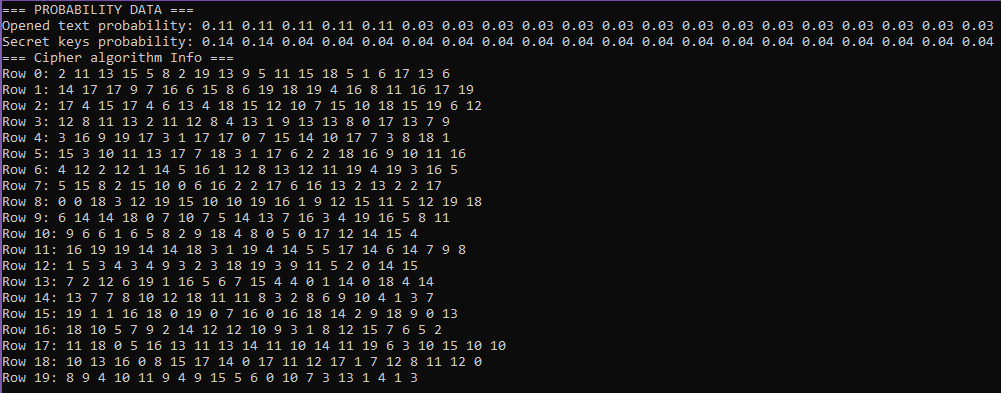
\includegraphics[width=0.8\textwidth]{/ReportPic/report_1.png}
        \end{minipage}
\end{figure}
\begin{figure}[!ht]
        \centering
        \begin{minipage}{\linewidth}
            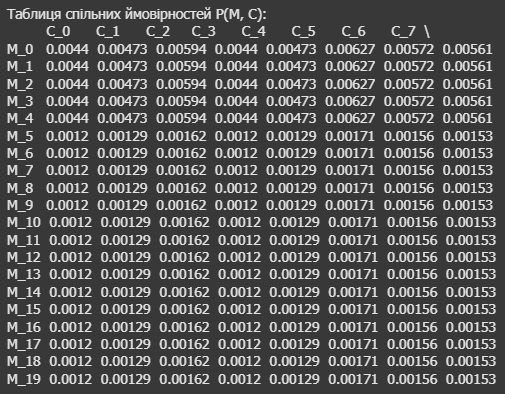
\includegraphics[width=0.4\textwidth]{/ReportPic/report_2.1.png}
        \end{minipage}
        \begin{minipage}{\linewidth}
            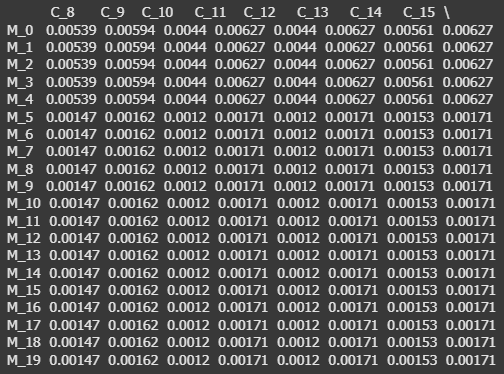
\includegraphics[width=0.4\textwidth]{/ReportPic/report_2.2.png}
        \end{minipage}
        \centering
        \begin{minipage}{\linewidth}
            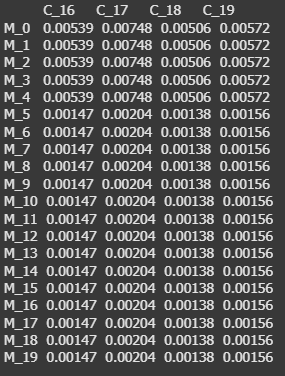
\includegraphics[width=0.15\textwidth]{/ReportPic/report_2.3.png}
        \end{minipage}
\end{figure}

Як результат роботи - видало перший ліпший $M_{i}$ (за критеріями підходить декілька)